\begin{figure}[!t]%
%   \makebox[\linewidth][c]{%
    \centering
    \begin{subfigure}[t]{0.74\textwidth}
        \centering
        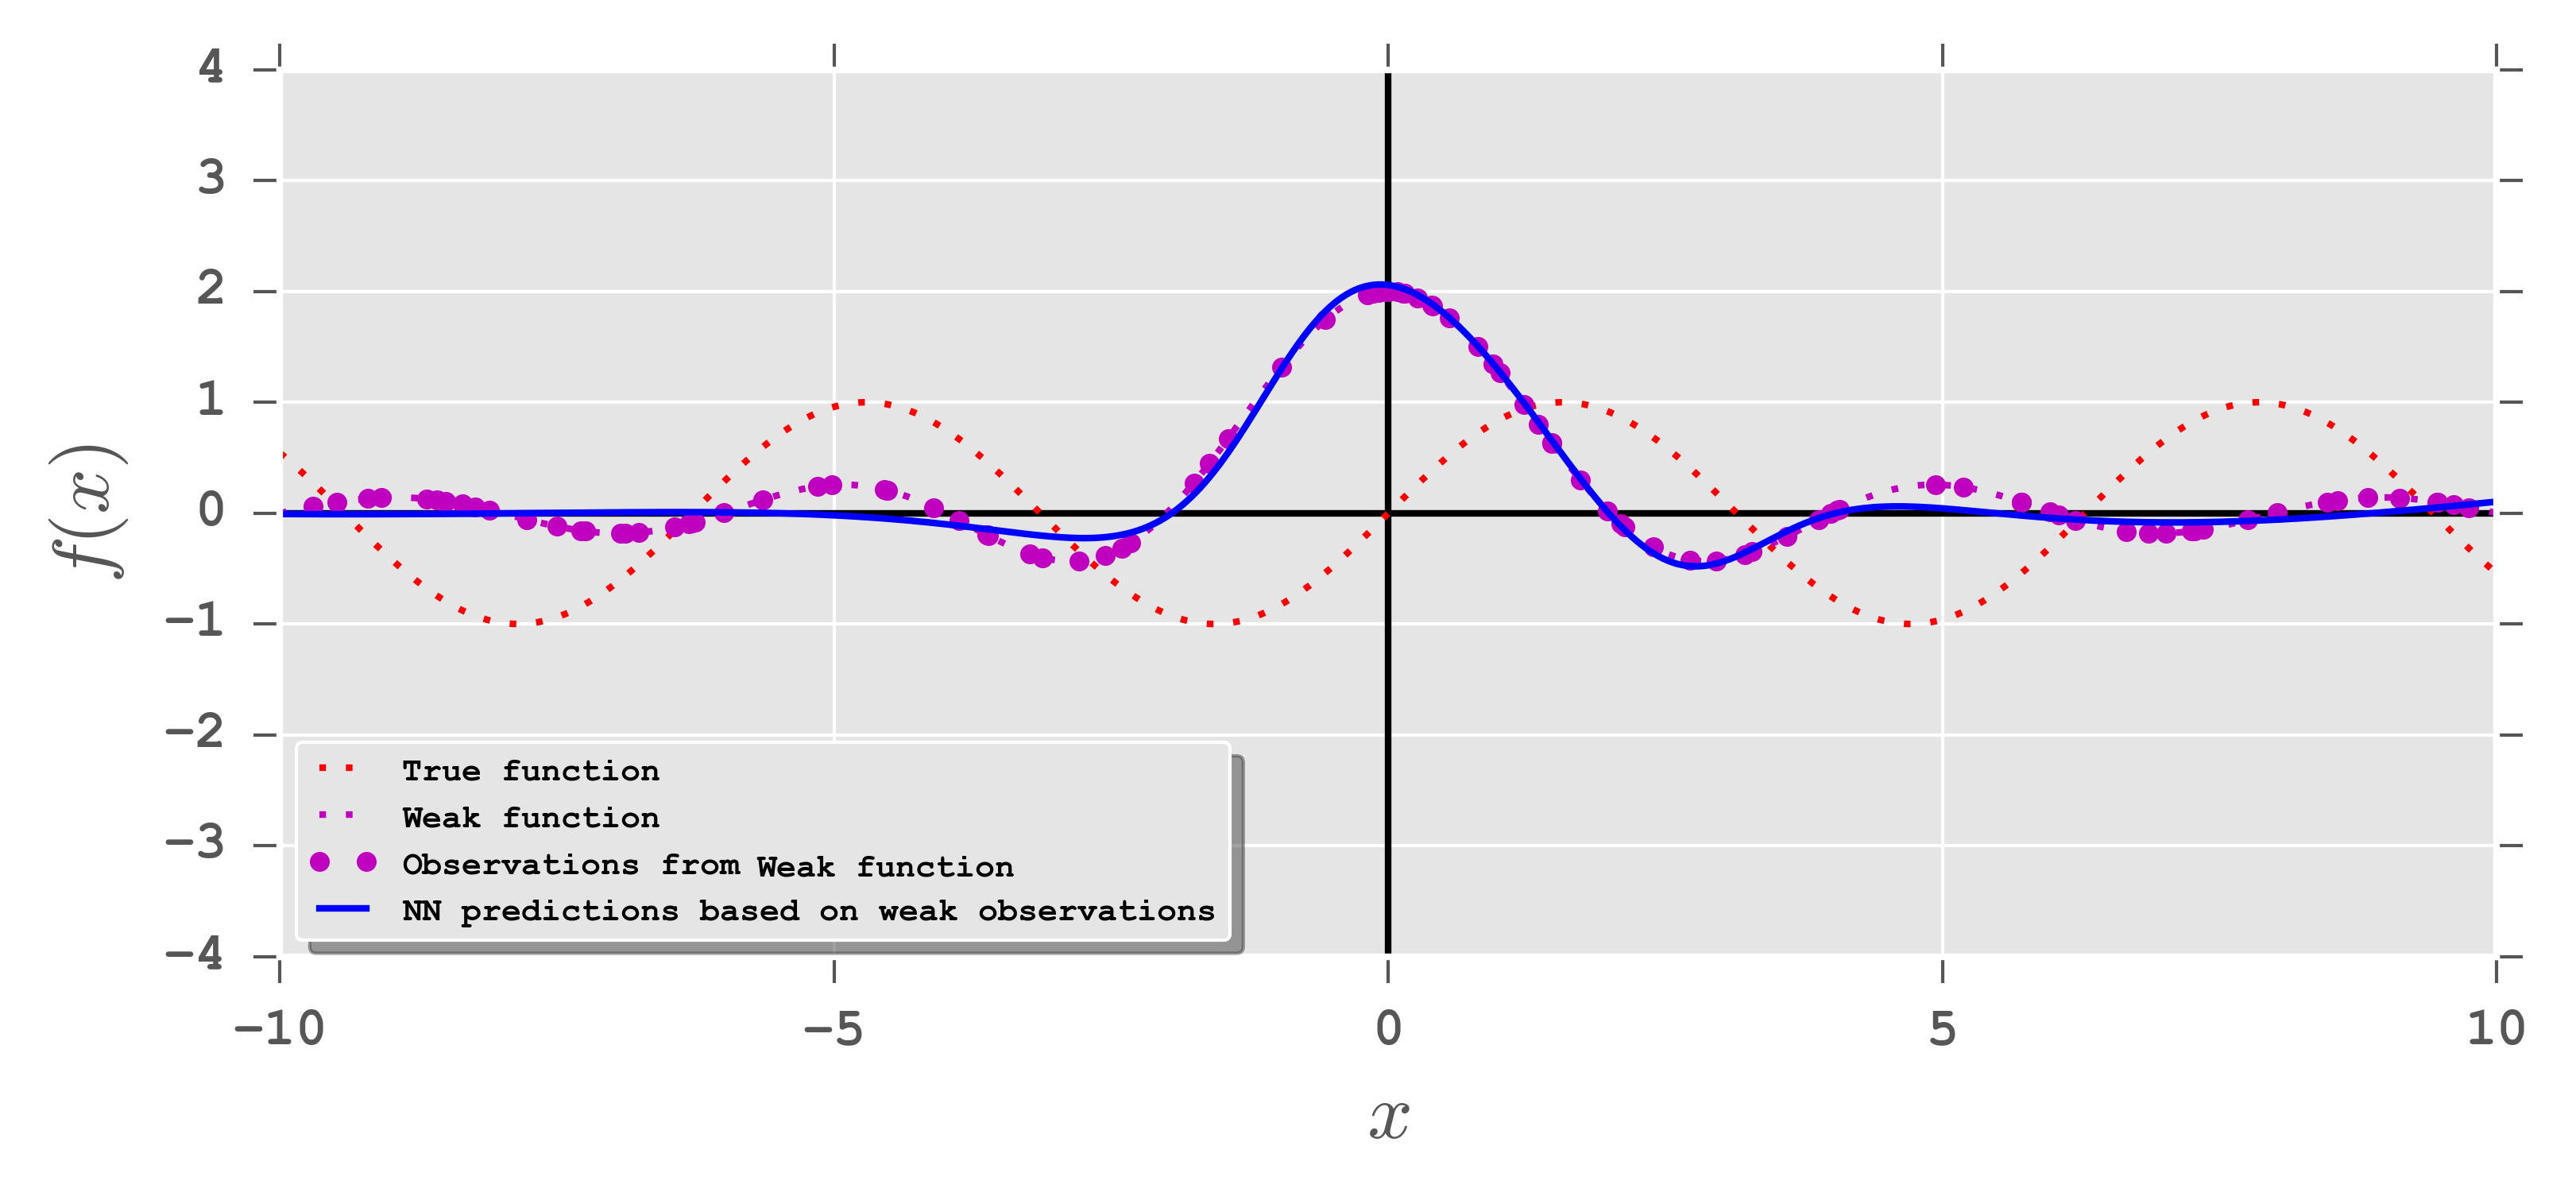
\includegraphics[trim={0 0.3cm 0 0},clip,width=1\textwidth]{03-part-02/chapter-05/figs_and_tables/fig_toy_ex_plot1.png}
        \caption{\label{fig:toy_plot1}Training \std on 100 samples from the weak function.}
    \end{subfigure}%
   \\
    \begin{subfigure}[t]{0.74\textwidth}
        \centering
        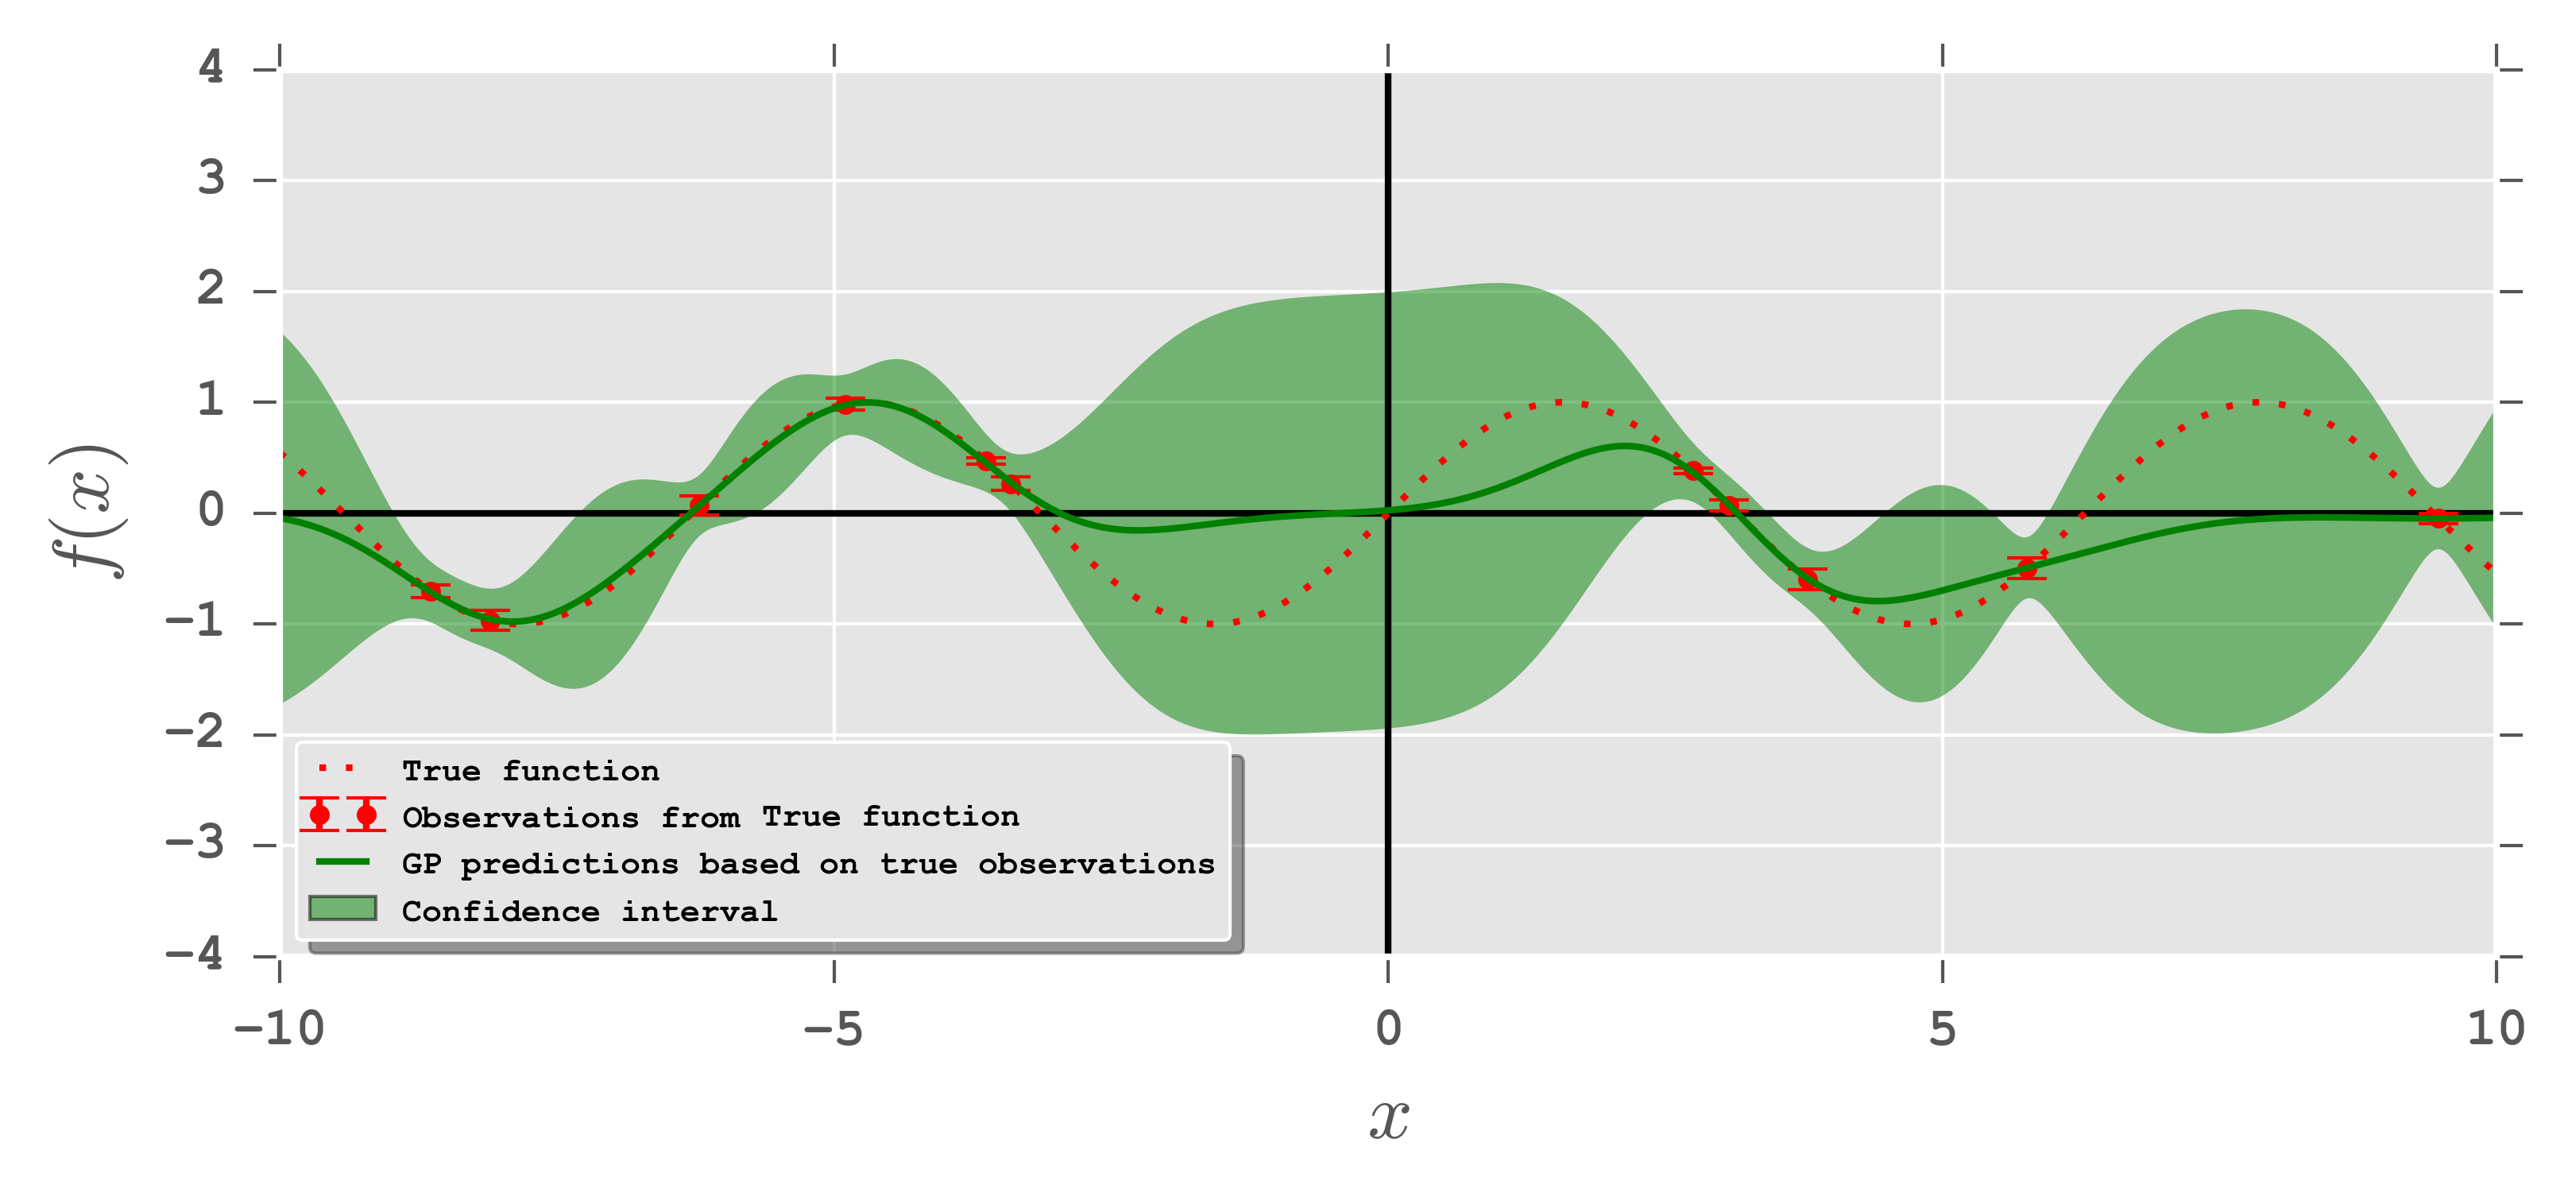
\includegraphics[trim={0 0.3cm 0 0},clip,width=1\textwidth]{03-part-02/chapter-05/figs_and_tables/fig_toy_ex_plot2.png}
        \caption{\label{fig:toy_plot2}Fitting \tch based on 10 observations from the true function.}
    \end{subfigure}%
    % }
    \\
    % \makebox[\linewidth][c]{%
    \begin{subfigure}[t]{0.74\textwidth}
        \centering
        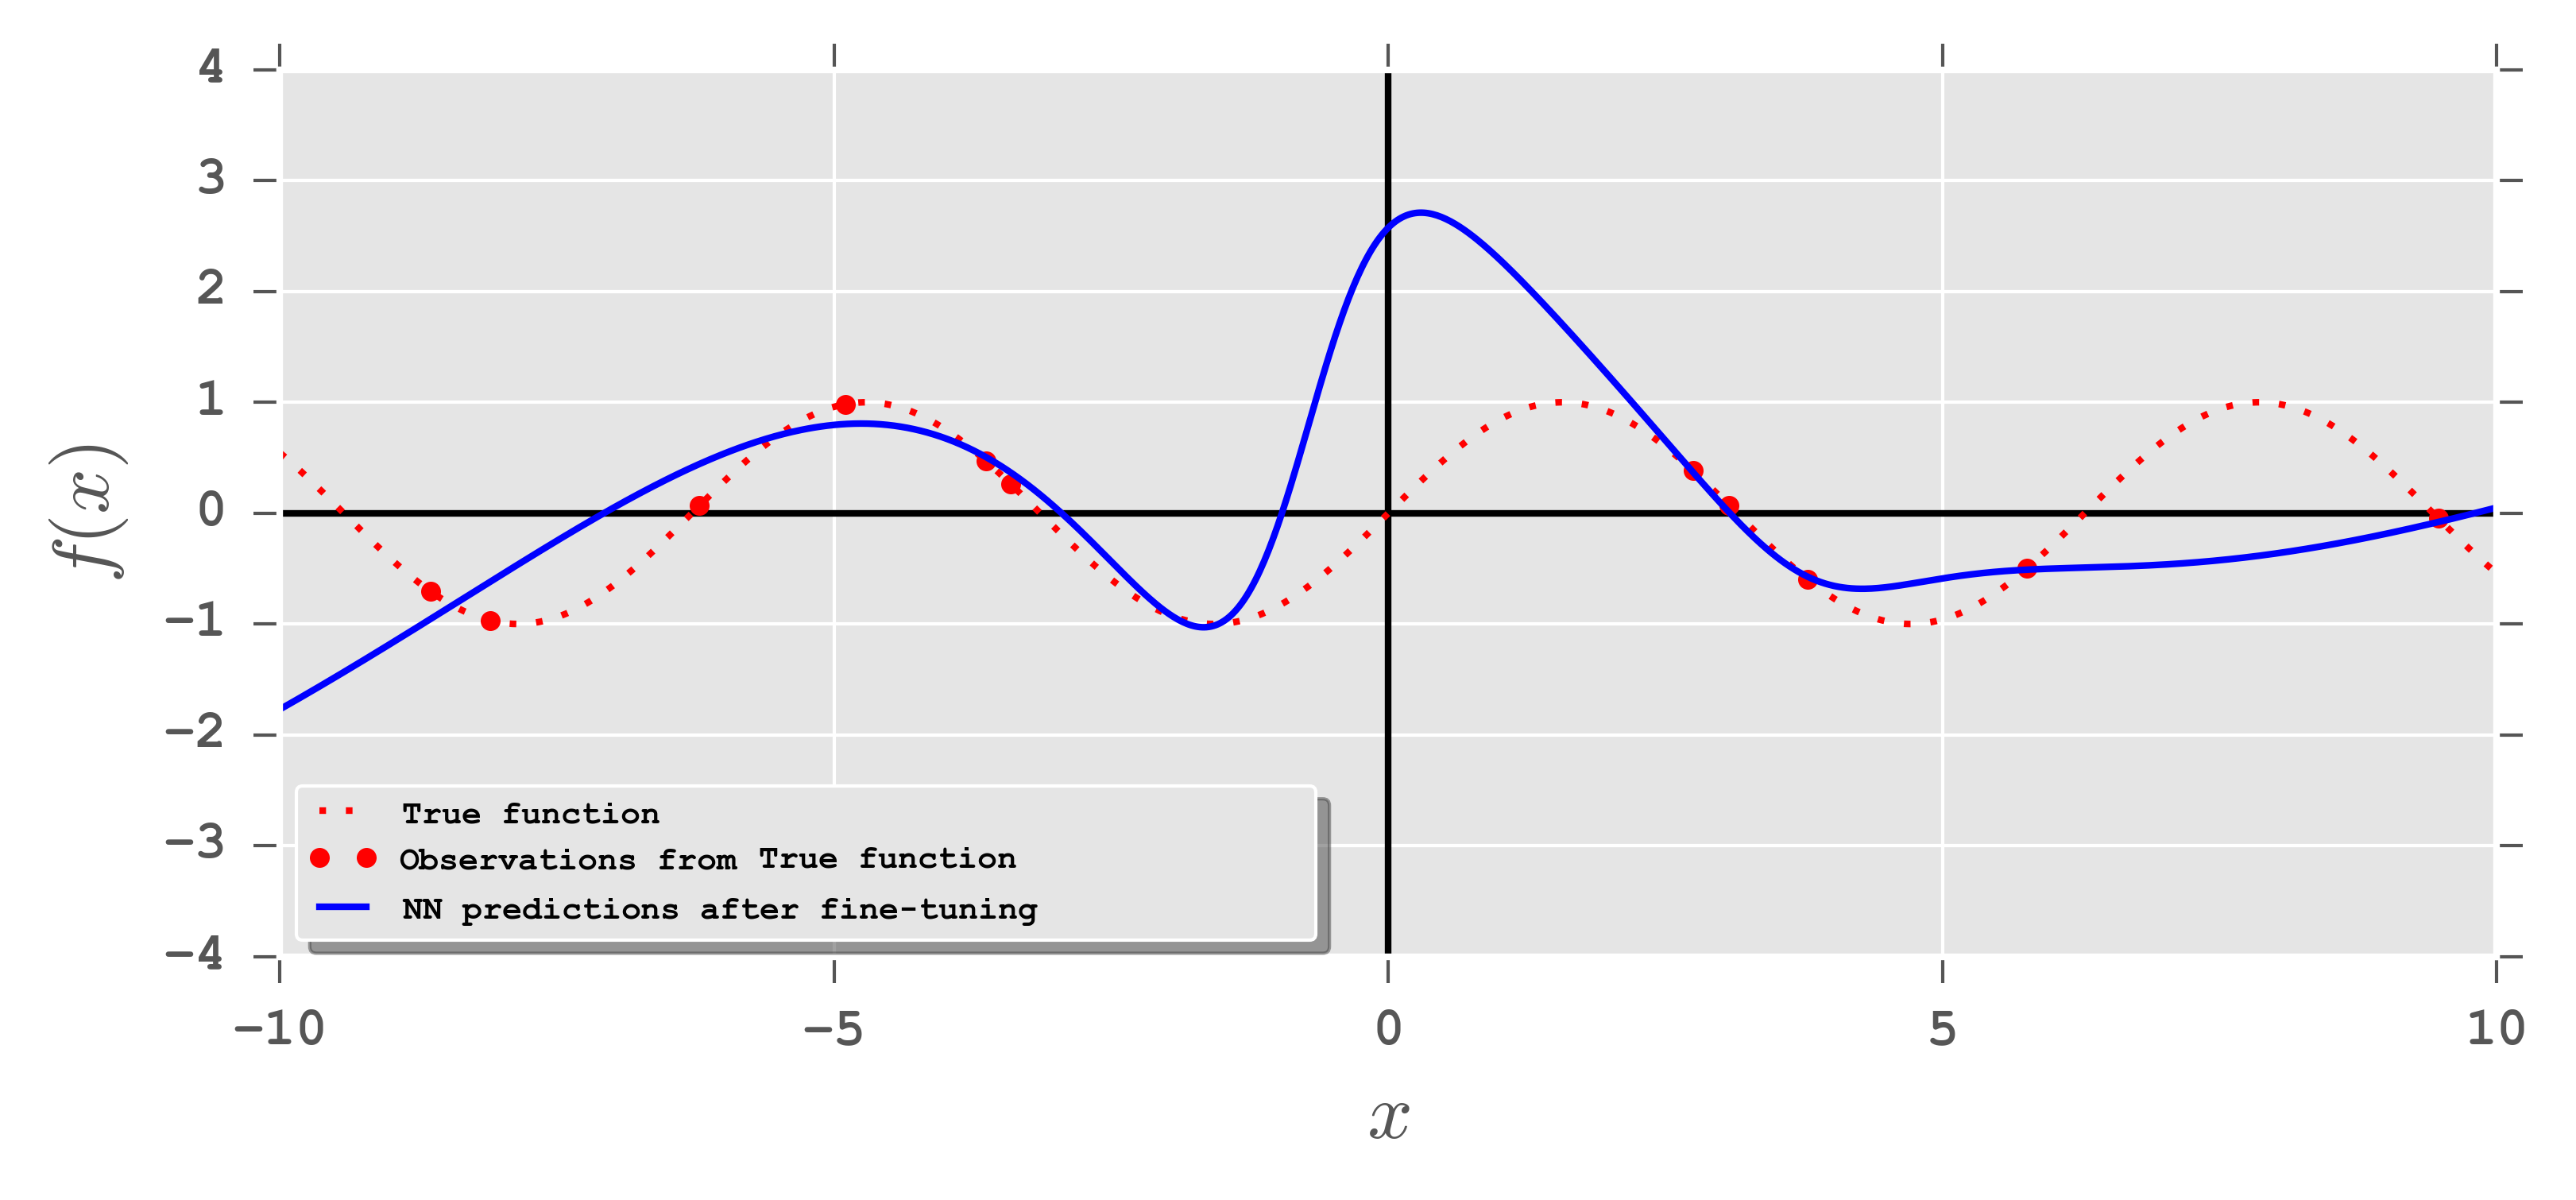
\includegraphics[trim={0 0.3cm 0 0},clip,width=1\textwidth]{03-part-02/chapter-05/figs_and_tables/fig_toy_ex_plot3.png}
        \caption{\label{fig:toy_plot3}Fine-tuning the \std based on observations from the true function.}
    \end{subfigure}%
    \\
    \begin{subfigure}[t]{0.74\textwidth}
        \centering
        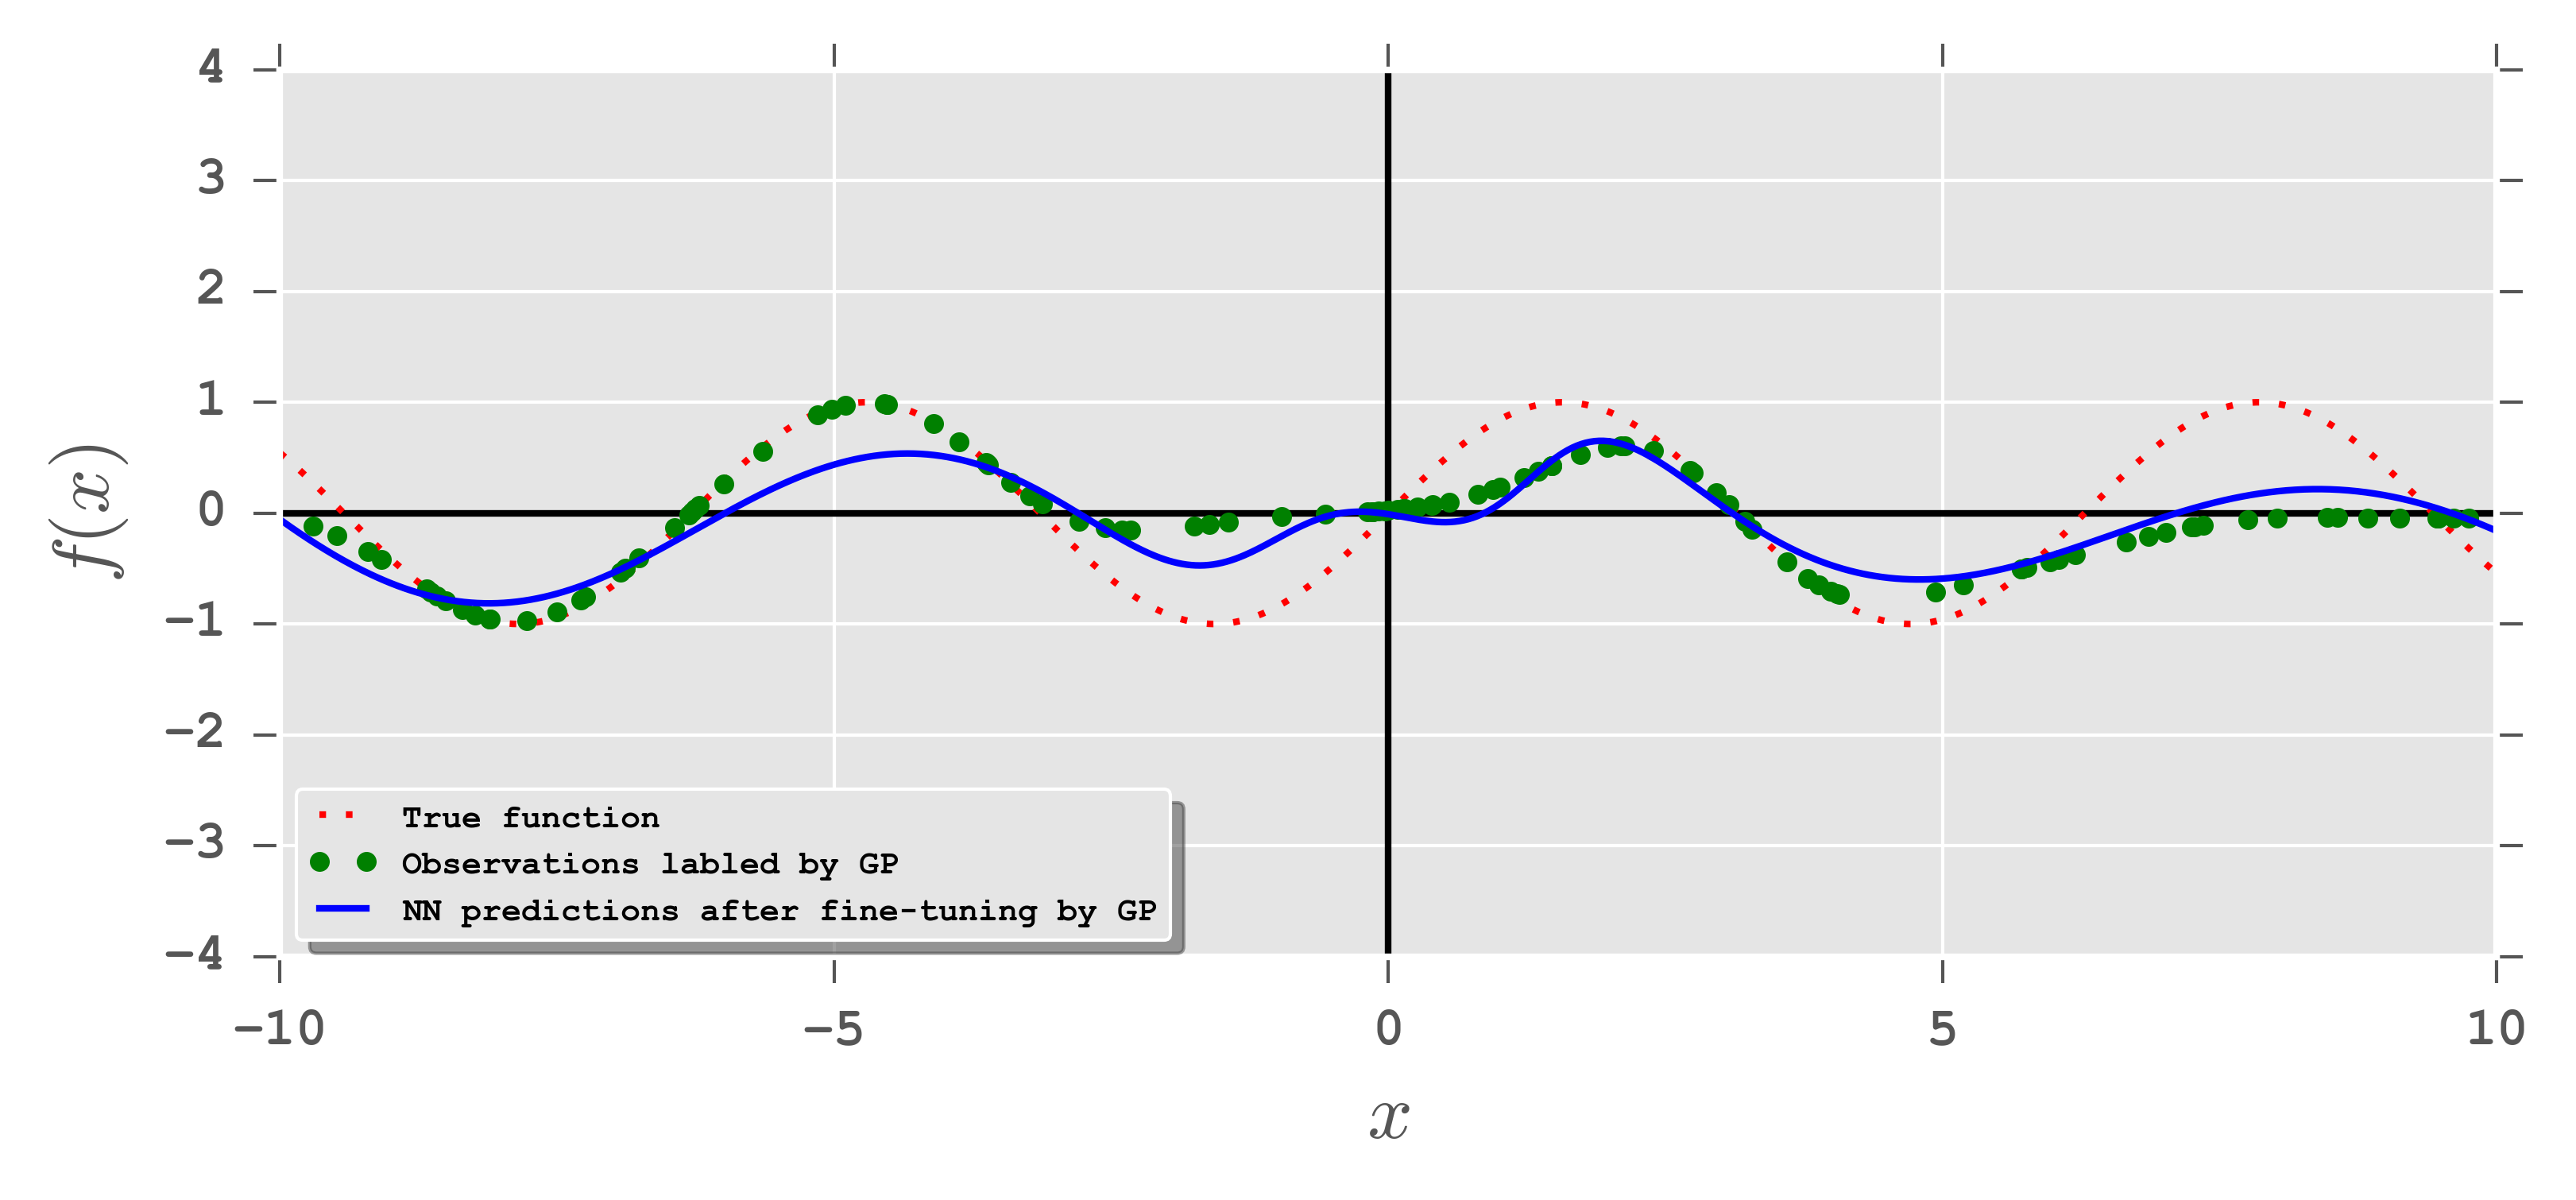
\includegraphics[trim={0 0.3cm 0 0},clip,width=1\textwidth]{03-part-02/chapter-05/figs_and_tables/fig_toy_ex_plot4.png}
        \caption{\label{fig:toy_plot4}Fine-tuning the \std based on label/confidence from \tch.}
    \end{subfigure}%
    % }
    \caption{Toy example: The true function we want to learn is $y = \sin(x)$ and the weak function is $y = 2 sinc(x)$.}
    \label{fig:toy}
\end{figure}